% !TEX root = ../paper.tex

\section{Algorithms}

\subsection{Sequential Algorithms}
\label{sec:seqalgs}

\subsubsection{Rank-2 NMF}
\label{sec:r2nmf}

Using the 2-block BCD approach for a rank-2 NMF yields NNLS subproblems of the form $\displaystyle \min_{\M[\bar]{H} \geq \M{0}} \|\M{W}\M[\bar]{H}^\Tra-\M{A}\|$ and $\min_{\M[\bar]{W} \geq \M{0}} \|\M{H}\M[\bar]{W}^\Tra-\M{A}^\Tra\|$.
In each case, the columns of the transposed variable matrix can be computed independently.
Considering the $i$th row of $\M[\bar]{H}$, for example, the NNLS problem to solve is
\begin{align*}
\begin{multlined}
\min_{\ME[\bar]{H}{i,1},\ME[\bar]{H}{i,2} \geq 0} \left\|\begin{bmatrix} \V{w}_1 & \V{w}_2 \end{bmatrix} \begin{bmatrix}\ME[\bar]{H}{i,1} \\ \ME[\bar]{H}{i,2} \end{bmatrix} - \V{A}_i \right\| \\ = \min_{\ME[\bar]{H}{i,1},\ME[\bar]{H}{i,2} \geq 0} \left\|\ME[\bar]{H}{i,1} \V{w}_1 + \ME[\bar]{H}{i,2} \V{w}_2 - \V{a}_i \right\|
\end{multlined}
\end{align*}
where $\V{w}_1$ and $\V{W}_2$ are the two columns of $\M{W}$ and $\V{a}_i$ is the $i$ column of $\M{A}$.
We note that there are four possibilities of solutions, as each of the two variables may be positive or zero.

As shown by Kuang and Park \cite{KP13}, determining which of the four possible solutions is feasible and optimal can be done efficiently by exploiting the following properties:
\begin{itemize}
	\item if the solution to the unconstrained least squares problem admits two positive values, it is the optimal solution to the nonnegatively constrained problem,
	\item if $\M{W}$ and $\M{A}$ are both nonnegative, then the candidate solution with two zero values is never (uniquely) optimal and can be discarded, and
	\item if the solution to the unconstrained problem does not admit two positive values, the better of the two remaining solutions can be determined by comparing $\V{a}_{j}^\Tra\V{w}_1 / \|\V{w}_1\|$ and $\V{a}_{j}^\Tra\V{w}_2 / \|\V{w}_2\|$.
\end{itemize}
If the unconstrained problem is solved via the normal equations, then the temporary matrices computed for the normal equations ($\M{W}^\Tra\M{W}$ and $\M{A}^\Tra\M{W}$) can be re-used to determine the better of the two solutions with a single positive variable.

\Cref{alg:r2nnls} implements this strategy for all rows of $\M{H}$ simultaneously.
It takes as input the matrices $\M{C}=\M{A}^\Tra\M{W}$ and $\M{G}=\M{W}^\Tra\M{W}$, first solves the normal equations for the unconstrained problem, and then chooses between the two alternate possibilities as necessary.
We note that each row of $\M{H}$ is independent, and therefore this algorithm is easily parallelized.
Solving for $\M{W}$ can be done using inputs $\M{C}=\M{A}\M{H}$ and $\M{G}=\M{H}^\Tra\M{H}$.

\begin{algorithm}
\caption{Rank-2 Nonnegative Least Squares Solve \cite{KP13}}
\label{alg:r2nnls}
\begin{algorithmic}[1]
	\Require{$\M{C}$ is $n\times 2$ and $\M{G}$ is $2\times 2$ and s.p.d.}
	\Function{$\M{H} =$ Rank2-NLS-Solve}{$\M{C},\M{G}$}
		\State $\M{H} = \M{C}\M{G}^{-1}$ \hfill \Comment{Solve unconstrained system}
		\For{$i=1$ to $n$}
			\If{$\ME{H}{i1} < 0$ or $\ME{H}{i2} < 0$}
				\State \Comment{Choose between single-variable solutions}
				\If{$\ME{C}{i1} / \sqrt{\ME{G}{11}}  < \ME{C}{i2} / \sqrt{\ME{G}{22}} $}
					\State $\ME{H}{i1} = 0$
					\State $\ME{H}{i2} = \ME{C}{i2} / \ME{G}{22}$
				\Else
					\State $\ME{H}{i1} = \ME{C}{i1} / \ME{G}{11}$
					\State $\ME{H}{i2} = 0$
				\EndIf
			\EndIf
		\EndFor
	\EndFunction
	\Ensure{$\displaystyle \M{H} = \argmin_{\M[\bar]{H} \geq \M{0}} \|\M{A}-\M{W}\M[\bar]{H}^\Tra\|$ is $n\times 2$ with $\M{C}=\M{A}^\Tra \M{W}$ and $\M{G}=\M{W}^\Tra\M{W}$}
\end{algorithmic}
\end{algorithm}

Given that the computational complexity of \Cref{alg:r2nnls} is $O(n)$ (or $O(m)$ when computing $\M{W}$), and the complexity of computing $\M{W}^\Tra\M{W}$ and $\M{H}^\Tra\M{H}$ is $O(m+n)$, the typical dominant cost of each iteration of Rank-2 NMF is that of computing $\M{A}^\Tra\M{W}$ and $\M{A}\M{H}$, which is $O(mn)$.

\subsubsection{Hierarchical Clustering}

A Rank-2 NMF can be used to partition the columns of the matrix into two parts.
In this case, the columns of the $\M{W}$ factor represent feature weights for each of the two latent components, and the strength of membership in the two components for each column of $\M{A}$ is given by the two values in the corresponding row of $\M{H}$.
We can determine part membership by comparing those values: if $\ME{H}{i1} > \ME{H}{i2}$, then column $i$ of $\M{A}$ is assigned to the first part, which is associated with feature vector $\V{w}_1$.
Membership can be determined by other metrics that also take into account balance across parts or attempt to detect outliers.

Given Rank-2 NMF as a splitting procedure, hierarchical clustering builds a binary tree such that each node corresponds to a subset of samples from the original data set and each node's children correspond to a 2-way partition of the node's samples.
In this way, the leaves form a partition of the original data, and the internal nodes specify the hierarchical relationship among clusters.
As the tree is built, nodes are split in order of their score, or relative value to the overall clustering of the data.
The process can be continued until a target number of leaves is produced or until all remaining leaves have a score below a given threshold.

A node's score can be computed in different ways.
For document clustering, Kuang and Park \cite{KP13} propose using modified normalized discounted cumulative gain, which measures how distinct a node's children are from each other using the feature weights associated with the node and its children.
For hyperspectral imaging data, Gillis et al. \cite{GKP15} propose using the possible reduction in overall NMF error if the node is split -- the difference in error between using the node itself or using its children.
We use the latter in our implementation.

In any case, a node's score depends on properties of its children, so the computation for a split must be done before the split is actually accepted.
To this end, we define a \emph{frontier} node to be a parent of leaves; these are nodes whose children have been computed but whose splits have not been accepted.
\Cref{fig:tree} depicts the classification of nodes into internal, frontier, and leaf nodes.
As the tree is built, the algorithm selects the frontier node with the highest score to split, though no computation is required to split the node.
When a frontier node split is accepted, it becomes an internal node and its children are split (so that their scores can be computed) and added to the set of frontier nodes.
When the algorithm terminates, the leaves are discarded and the frontier nodes become the leaves of the output tree.

\begin{figure}
%!TEX root = ../paper.tex

\centering
\scalebox{.75}{
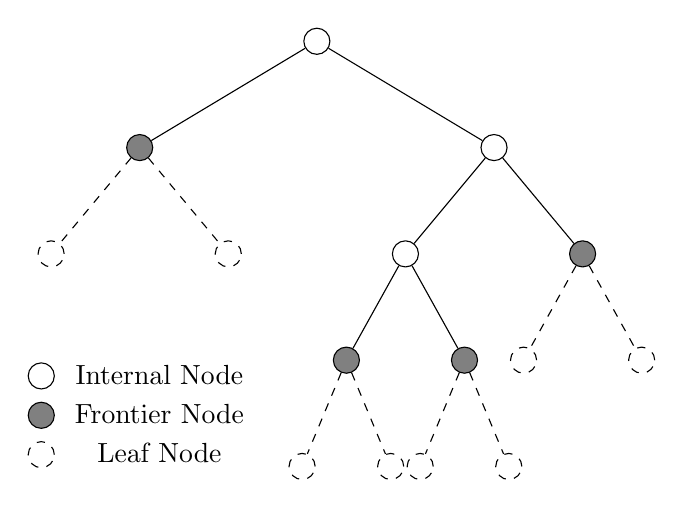
\begin{tikzpicture}[scale=.9,level/.style={sibling distance=50mm/#1}]
\node [circle,draw] (z) {}
  child {node [circle,draw,fill=gray] (a) {}
    child[dashed] {node [circle,draw,dashed] (b) {}}
    child[dashed] {node [circle,draw,dashed] (g) {}}
  }
  child {node [circle,draw] (j) {}
    child {node [circle,draw] (k) {}
      child {node [circle,draw,fill=gray] (o) {}
        child[dashed] {node [circle,draw,dashed] (x) {}}
        child[dashed] {node [circle,draw,dashed] (y) {}}
      }
      child {node [circle,draw,fill=gray] (p) {}
        child[dashed] {node [circle,draw,dashed] (x) {}}
        child[dashed] {node [circle,draw,dashed] (y) {}}
      }
    }
  child {node [circle,draw,fill=gray] (l) {}
    child[dashed] {node [circle,draw,dashed] (c) {}}
    child[dashed] {node [circle,draw,dashed] (d) {}}
  }
};

\node [shift={(-3.5,-4.25)},circle,draw,label={[xshift=1.5cm, yshift=-0.4cm] Internal Node}] (leg1) {};
\node [shift={(-3.5,-4.75)},circle,draw,fill=gray,label={[xshift=1.5cm, yshift=-0.4cm] Frontier Node}] (leg1) {};
\node [shift={(-3.5,-5.25)},circle,draw,dashed,label={[xshift=1.5cm, yshift=-0.4cm] Leaf Node}] (leg1) {};
\end{tikzpicture}
}
\caption{Hierarchy node classification}
\label{fig:tree}
\end{figure}

Our hierarchical clustering algorithm is presented in \Cref{alg:hiernmf2} and follows that of Kuang and Park \cite{KP13}.
Each node includes a field $\M{A}$, which is a subset of columns (samples) of the original data, a feature vector $\V{w}$, which is its corresponding column of the $\M{W}$ matrix from its parent's Rank-2 NMF, a score, and pointers to its left and right children.
A priority queue $\cal Q$ tracks the frontier nodes so that the node with the highest score is split at each step of the algorithm.
We use a target number of leaf clusters $k$ as the termination condition.
When a node is selected from the priority queue, it is removed from the set of frontier nodes and its children are added.

\begin{algorithm}
\caption{Hierarchical Clustering \cite{KP13}}
\label{alg:hiernmf2}
\begin{algorithmic}[1]
	\Require{$\M{A}$ is $m\times n$, $k$ is target number of leaf clusters}
	\Function{${\cal T} =$ Hier-R2-NMF}{$\M{A}$}
		\State ${\cal R} = \text{node}(\M{A})$ \hfill \Comment{create root node}
		\State \textsc{Split}$({\cal R})$
		\State inject$({\cal Q},{\cal R}.\text{left})$ \hfill \Comment{create priority queue}
		\State inject$({\cal Q},{\cal R}.\text{right})$ \hfill \Comment{of frontier nodes}
		\While{size$({\cal Q}) < k$}
			\State ${\cal N} = \text{eject}({\cal Q})$ \hfill \Comment{frontier node with max score}
			\State \textsc{Split}$({\cal N}.\text{left})$ \hfill \Comment{split left child}
			\State inject$({\cal Q},{\cal N}.\text{left})$ \hfill \Comment{and add to $\cal Q$}
			\State \textsc{Split}$({\cal N}.\text{right})$ \hfill \Comment{split right child}
			\State inject$({\cal Q},{\cal N}.\text{right})$ \hfill \Comment{and add to $\cal Q$}
		\EndWhile
	\EndFunction
	\Ensure{$\cal{T}$ is binary tree rooted at $\cal R$ with $k$ frontier nodes, each node has subset of cols of $\M{A}$ and feature vector $\V{w}$}
\end{algorithmic}
\end{algorithm}

The splitting procedure is specified in \Cref{alg:split}.
After the Rank-2 NMF is performed, the $\M{H}$ factor is used to determine part membership, and the columns of the $\M{W}$ factor are assigned to the child nodes.
The score of the node is computed as the reduction in overall NMF error if the node is split, which can be computed from the principal singular values of the subsets of columns of the node and its children, as given in \Cref{line:score}.
The principal singular values of the children are computed via the power method.
Note that the principal singular value of the node itself need not be recomputed as it was needed for its parent's score.


\begin{algorithm}
\caption{Node Splitting via Rank-Two NMF}
\label{alg:split}
\begin{algorithmic}[1]
	\Require{$\cal N$ has a subset of columns given by field $\M{A}$}
	\Function{Split}{$\cal N$}
		\State $[\M{W},\M{H}] = \textsc{Rank2-NMF}({\cal N}.\M{A})$ \hfill \Comment{split $\cal N$}
		\State partition ${\cal N}.\M{A}$ into $\M{A}_1$ and $\M{A}_2$ using $\M{H}$
		\State ${\cal N}.\text{left} = \text{node}(\M{A}_1,\V{W}_1)$ \hfill \Comment{create left child}
		\State ${\cal N}.\text{right} = \text{node}(\M{A}_2,\V{W}_2)$ \hfill \Comment{create right child}
		\State ${\cal N}.\text{score} = \sigma_1^2(\M{A}_1) + \sigma_1^2(\M{A}_2) - \sigma_1^2({\cal N}.\M{A})$ \label{line:score}
	\EndFunction
	\Ensure{$\cal{N}$ has two children and a score}
\end{algorithmic}
\end{algorithm}

\subsection{Parallelization}
\label{sec:paralgs}

In this section, we consider the options for parallelizing Hierarchical Rank-2 NMF Clustering (\Cref{alg:hiernmf2}) and provide an analysis for our approach.
The running time of an algorithm is data dependent because not only does each Rank-2 NMF computation require a variable number of iterations, but also the shape of the tree can vary from a balanced binary tree with $O(\log k)$ levels to a tall, flat tree with $O(k)$ levels.
For the sake of analysis, we will assume a fixed number of NMF iterations for every node of the tree and we will analyze the cost of complete levels.

The first possibility for parallelization is across the nodes of the tree, as each Rank-2 NMF split is independent.
We choose not to parallelize across nodes in the tree for two reasons.
The first reason is that while the NMF computations are independent, choosing which nodes to split may depend on global information.
In particular, when the global target is to determine $k$ leaf clusters, the nodes must be split in order of their scores, which leads to a serialization of the node splits.
This serialization might be relaxed using speculative execution, but it risks performing unnecessary computation.
If the global target is to split all nodes with sufficiently high scores, then this serialization is also avoided and node splits become truly independent.
We choose not to parallelize in this way to remain agnostic to the global stopping criterion.

The second reason is that parallelizing across nodes requires redistribution of the input data.
Given a node split by $\hat p$ processors, in order to assign disjoint sets of processors to each child node, each of the $\hat p$ processors would have to redistribute their local data, sending data for samples not in their child's set and receiving data for those in their child's set.
The communication would be data dependent, but on average, each processor would communicate half of its data in the redistribution set, which could have an all-to-all communication pattern among the $\hat p$ processors.
For a node with $\hat n$ columns, the communication cost would be at least $O(m\hat n/ \hat p)$ words, which is much larger than the communication cost per iteration of Parallel Rank-2 NMF, as we will see in \Cref{sec:analysis}.

By choosing not to parallelize across nodes in the tree, we employ all $p$ processors on each node, and split nodes in sequence.
The primary computations used to split a node are the Rank-2 NMF and the score computation, which is based on an approximation of the largest singular value.
We use an alternating-updating algorithm for Rank-2 NMF as described in \Cref{sec:prelim}, and we parallelize it following the methodology proposed in \cite{EH+19-TR} and presented in \Cref{alg:parrank2nmf}.

The communication cost of the algorithm depends on the parallel distribution of the input matrix data $\M{A}$.
In order to avoid redistribution of the matrix data, we choose a 1D row distribution so that each processor owns a subset of the rows of $\M{A}$.
Because the clustering partition splits the columns of $\M{A}$, each processor can partition its local data into left and right children to perform the split without any interprocessor communication.
If we use a 2D distribution for a given node, then because the partition is data dependent, a data redistribution is required in order to obtain a load balanced distribution of both children.
\Cref{fig:split} presents a visualization of the node-splitting process using a 1D processor distribution.
In the following subsections, we describe the parallel algorithms for Rank-2 NMF and approximating the principal singular value given this 1D data distribution and analyze their complexity in the context of the hierarchical clustering algorithm.

\begin{figure}
%!TEX root = ../paper.tex

\newcommand{\lightred}{red!75}
\newcommand{\lightblue}{blue!75}
\newcommand{\offset}{.1}

\begin{tikzpicture}

% draw A
\fill[\lightred] (0,0) rectangle ++(0.5,4);
\fill[\lightblue] (0.5,0) rectangle ++(1.25,4);
\fill[\lightred] (1.75,0) rectangle ++(1.25,4);
\fill[\lightblue] (3,0) rectangle ++(1,4);
\draw[thick,dashed,xscale=4,yscale=4/3] (0,0) grid ++(1,3);
\draw[very thick] (0,0) rectangle (4,4);
\node at (2,-3*\offset) {$\M{A}$};

% draw W
\draw[fill=\lightred,shift={(-.5,0)}] (0,0) rectangle ++ (.15,4);
\draw[fill=\lightblue,shift={(-.5,0)}] (.15,0) rectangle ++ (.15,4);
\draw[thick,shift={(-.5,0)},xscale=.15,yscale=4] (0,0) grid ++(2,1);
\node at (-.5+.15,-3*\offset) {$\M{W}$};

% draw H
\draw[thick,shift={(0,4.1)},xscale=4,yscale=.15] (0,0) grid ++(1,2);
\node at (4+4*\offset,4.3) {$\M{H}^\Tra$};
\draw[fill=\lightred,shift={(0,4.1)}] (0,.15) rectangle ++(.5,.15);
\draw[fill=\lightblue,shift={(0,4.1)}] (.5,0) rectangle ++(1.25,.15);
\draw[fill=\lightred,shift={(0,4.1)}] (1.75,.15) rectangle ++(1.25,.15);
\draw[fill=\lightblue,shift={(0,4.1)}] (3,0) rectangle ++(1,.15);

\begin{scope}[shift={(-1,-6)}]
	% draw A_1 and w_1
	\draw[very thick,fill=\lightred] (0,0) rectangle ++(2.25,4);
	\draw[thick,dashed,xscale=2.25,yscale=4/3] (0,0) grid ++(1,3);
	\node at (1.125,-3*\offset) {$\M{A}_1$};
	\draw[thick,fill=\lightred] (-.5,0) rectangle ++(.15,4);
	\node at (-.5+.15,-3*\offset) {$\V{W}_1$};
	
	% draw A_2 and w_2
	\draw[very thick,fill=\lightblue] (5,0) rectangle ++(1.75,4);
	\draw[thick,dashed,shift={(5,0)},xscale=1.75,yscale=4/3] (0,0) grid ++(1,3);
	\node at (5.875,-3*\offset) {$\M{A}_2$};
	\draw[thick,,fill=\lightblue,shift={(5,0)}] (-.5,0) rectangle ++(.15,4);
	\node at (5-.5+.15,-3*\offset) {$\V{W}_2$};
\end{scope}

% draw arrows to A_1 and w_1
% TODO: make these arrows prettier
\draw[thick] (0.25,-\offset) parabola (.125,-0.5);
\draw[thick] (2.25,-\offset) parabola (.125,-0.5);
\draw[thick,->] (.125,-0.5) parabola (.125,-2+\offset);
\draw[thick,->] (-.5+.075,-\offset) parabola (-1.5+.075,-2+\offset);

% draw arrows to A_2
% TODO: make these arrows prettier
\draw[thick] (1,-\offset) parabola (4.375,-0.5);
\draw[thick] (3.5,-\offset) parabola (4.375,-0.5);
\draw[thick,->] (4.375,-0.5) parabola (4.875,-2+\offset);
\draw[thick,->] (-.5+.225,-\offset) parabola (3.5+.075,-2+\offset);

\end{tikzpicture}

\caption{Parallel splitting using Rank-2 NMF and 1D processor distribution.  A Rank-2 NMF computes factor matrices $\M{W}$ and $\M{H}$ to approximate $\M{A}$, the values of $\M{H}$ are used to determine child membership of each column (either red or blue), and the corresponding column of the $\M{W}$ matrix represents the part's feature weighting.  The 1D distribution is depicted for 3 processors to show that the splitting requires no interprocessor redistribution as the children are evenly distributed identically to the parent.}
\label{fig:split}
\end{figure}

\subsubsection{Algorithms}

\paragraph{\emph{Parallel Rank-2 NMF}}

\Cref{alg:parrank2nmf} presents the parallelization of an alternating-updating scheme for NMF that uses the exact rank-2 solve algorithm presented in \Cref{alg:r2nnls} to update each factor matrix.
The algorithm computes the inputs to the rank-2 solves in parallel and then exploits the parallelism across rows of the factor matrix so that each processor solves for a subset of rows simultaneously.
The distribution of all matrices is 1D row distribution, so that each processor owns a subset of the rows of $\M{A}$, $\M{W}$, and $\M{H}$.
We use the notation $\M[\hat]{A}$ to refer to the $(m/p) \times n$ local data matrix and $\M[\hat]{W}$ and $\M[\hat]{H}$ to refer to the $(m/p) \times 2$ and $(n/p)\times 2$ local factor matrices.
With this distribution, the computation of $\M{W}^\Tra\M{W}$ and $\M{H}^\Tra\M{H}$ each is done via local multiplication followed by a single all-reduce collective.
All processors own the data they need to compute their contribution to $\M{A}^\Tra \M{W}$; in order to distribute the result to compute the rows $\M{H}$ independently, a reduce-scatter collective is used to sum and simultaneously distribute across processors.
To obtain the data needed to compute $\M[\hat]{W}$, each processor must access all of $\M{H}$, which is performed via an all-gather collective.
The iteration progresses until a convergence criterion is satisfied.
For performance benchmarking we use a fixed number of iterations, and in practice we use relative change in objective function value (residual norm).

\begin{algorithm}
\caption{Parallel Rank-2 NMF}
\label{alg:parrank2nmf}
\begin{algorithmic}[1]
	\Require{$\M{A}$ is $m\times n$ and row-distributed across processors so that $\M[\hat]{A}$ is local $(m/p)\times n$ submatrix}
	\Function{$[\M{W},\M{H}] =$ Parallel-Rank2-NMF}{$\M{A}$}
		\State Initialize local $\M[\hat]{W}$ randomly
		\While{not converged}
			\State \Comment{Compute $\M{H}$}
			\State $\M[\hat]{G}_W = \M[\hat]{W}^\Tra \M[\hat]{W}$
			\State $\M{G}_W = \textsc{All-Reduce}(\M[\hat]{G})$
			\State $\M[\hat]{B} = \M[\hat]{A}^\Tra \M[\hat]{W}$ %\hfill \Comment{local matrix multiplication}
			\State $\M[\hat]{C} = \textsc{Reduce-Scatter}(\M[\hat]{B})$
			\State $\M[\hat]{H} = \textsc{Rank2-NLS-Solve}(\M[\hat]{C},\M{G}_W)$
			\State \Comment{Compute $\M{W}$}
			\State $\M[\hat]{G}_H = \M[\hat]{H}^\Tra \M[\hat]{H}$
			\State $\M{G}_H = \textsc{All-Reduce}(\M[\hat]{G}_H)$
			\State $\M{H} = \textsc{All-Gather}(\M[\hat]{H})$
			\State $\M[\hat]{D} = \M[\hat]{A} \M{H}$ %\hfill \Comment{local matrix multiplication}
			\State $\M[\hat]{W} = \textsc{Rank2-NLS-Solve}(\M[\hat]{D},\M{G}_H)$
		\EndWhile
	\EndFunction
	\Ensure{$\M{A} \approx \M{W}\M{H}^\Tra$ with $\M{W}$, $\M{H}$ row-distributed}
\end{algorithmic}
\end{algorithm}

\paragraph{\emph{Parallel Power Method}}

In order to compute the score for a frontier node, we use the difference between the principal singular value of the matrix columns of the node and the sum of those of its children.
Thus, we must determine the principal singular value of every node in the tree once, including leaf nodes.
We use the power method to approximate it, repeatedly applying $\M{A}\M{A}^\Tra$ to a vector until it converges to the leading right singular vector.
We present the power method in \Cref{alg:parpowmeth}.
Note that we do not normalize the approximate left singular vector so that the computed value approximates the square of the largest singular value.

Given the 1D distribution, only one communication collective is required for the pair of matrix-vector multiplications.
That is, the approximate right singular vector $\V{v}$ is redundantly owned on each processor, and the approximate left singular vector $\V{u}$ is distributed across processors.
Each processor can compute its local $\V[\hat]{u}$ from $\V{v}$ without communication and use the result for its contribution to $\V{v}=\M{A}^\Tra \V{u}$.
An all-reduce collective is used to obtain a copy of $\V{v}$ on every processor for the next iteration, and the norm is redundantly computed without further communication.
We used the relative change in $\sigma$ as the stopping criterion for benchmarking.

\begin{algorithm}
\caption{Parallel Power Method}
\label{alg:parpowmeth}
\begin{algorithmic}[1]
	\Require{$\M{A}$ is $m\times n$ and row-distributed across processors so that $\M[\hat]{A}$ is local $(m/p)\times n$ submatrix}
	\Function{$\sigma =$ Parallel-Power-Method}{$\M{A}$}
		\State Initialize $\V{v}$ randomly and redundantly
		\While{not converged}
			\State $\V[\hat]{u} = \M[\hat]{A} \V{v}$
			\State $\V[\hat]{z} = \M[\hat]{A}^\Tra \V[\hat]{u}$
			\State $\V{v} = \textsc{All-Reduce}(\V[\hat]{z})$
			\State $\sigma = \|\V{v}\|$
			\State $\V{v} = \V{v}/\sigma$
		\EndWhile
	\EndFunction
	\Ensure{$\sigma \approx \sigma_1^2(\M{A})$ is  redundantly owned by all procs}
\end{algorithmic}
\end{algorithm}

